\documentclass{beamer}

\usepackage{graphicx}
\usepackage{tikz}

\title{The Scrum Method}
\author{Jimmy Mousel, Colin Holler, Dimitri Klockenbring, Jérémie Muzet, Céline Van Landeghem}
\date{}
\begin{document}


\frame{\titlepage}


\begin{frame}
    \frametitle{First slide}
    
    This is a text in second frame. 
    For the sake of showing an example.
    
    \begin{itemize}
     \item<1-> Text visible on slide 1
     \item<2-> Text visible on slide 1
     \item<3> Text visible on slide 1
     \item<4-> Text visible on slide 1
    \end{itemize}
    
\end{frame}

\begin{frame}
    \frametitle{Second slide}

    \begin{center}

	% à ordonner correctement :%
	% l'origine est en bas à gauche %
	% juste à gauche de "rectangle" on met les coordonnées du coin inf gauche
	% juste à droite de "rectangle" on met les coordonnées du point sup droit
        % Dans les chevrons après "draw" on indique à quel moment ça s'affiche
	
	\begin{tikzpicture}
            \node[anchor=south west,inner sep=0] at (0,0) {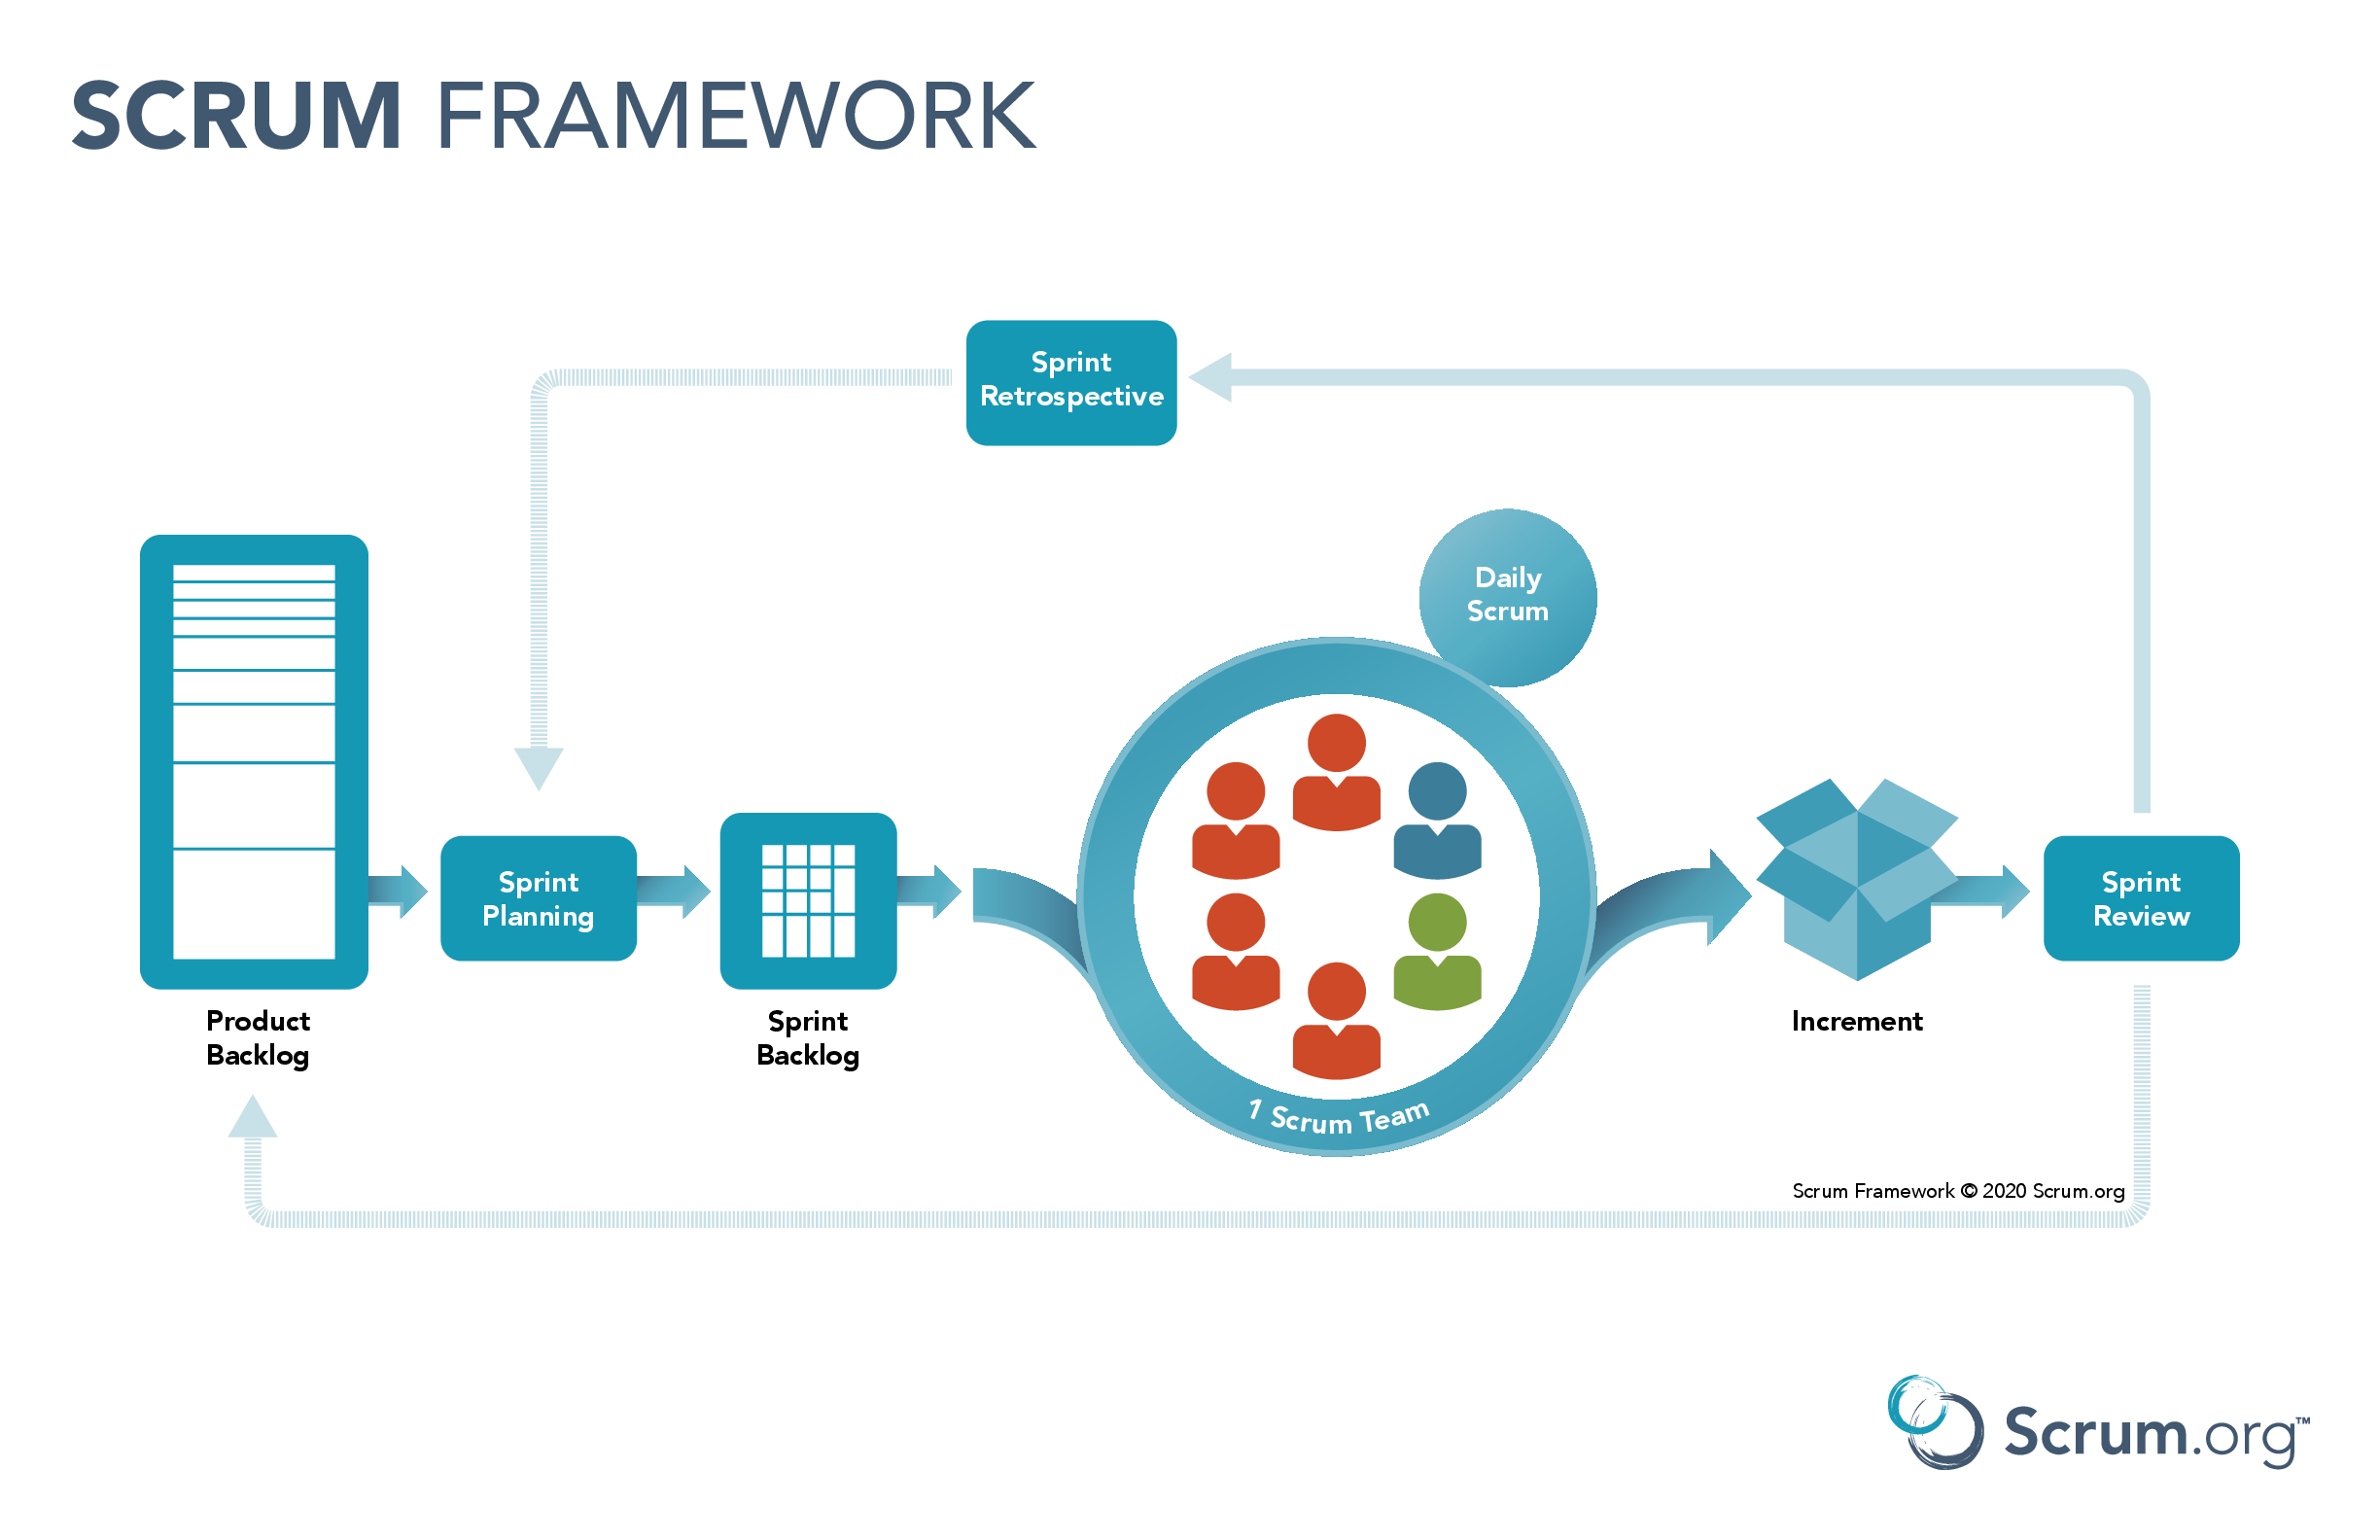
\includegraphics[width=1\textheight]{Images/Scrumorg-Scrum-Framework}};
            \draw<1>[red,ultra thick,rounded corners] (0.4,1.8) rectangle (1.6,4.2);
            \draw<2>[red,ultra thick,rounded corners] (1.6,2.1) rectangle (2.8, 3);
	    \draw<3>[red,ultra thick,rounded corners] (2.7,1.8) rectangle (3.7, 3);
	    \draw<4>[red,ultra thick,rounded corners] (3.7,4.2) rectangle (4.8, 5);
	    \draw<5>[red,ultra thick,rounded corners] (5.6,3.3) rectangle (6.4, 4.2);
	    \draw<6>[red,ultra thick,rounded corners] (6.9,1.9) rectangle (7.9, 3.2);
	    \draw<7>[red,ultra thick,rounded corners] (8,2.1) rectangle (9, 3);
        \end{tikzpicture}
    \end{center}
    
\end{frame}

\begin{frame}
    \frametitle{Advantages and Disadvantages}

    
\end{frame}

\begin{frame}
    \frametitle{SCRUM and GitHub}
 
    \begin{itemize}
    \color{gray}
    \item[•] Sprints
    \item[•] \textcolor{black}{Issues}
    \item[•] GitScrum
    \end{itemize}
    
    
\end{frame}

\begin{frame}
    \frametitle{Bibliography}

	\begin{thebibliography}{10}
	
	\bibitem{ScrumOnGithub}
	\textit{Software Development Practices with GitHub} \\
	\texttt{https://www.scrumassembly.org/Library/ScrumMastery/ISM/\\
	International+Scrum\%E2\%84\%A2/Software+Development+Practices+with+GitHub}
	
	\bibitem{agile}
	\textit{How To Use GitHub for Agile Project Management} \\
	\texttt{https://blog.zenhub.com/how-to-use-github-agile-project-management/}

	\end{thebibliography}
    
    
\end{frame}

\end{document}